\section{$n$阶展开方法及其应用}
\begin{frame}
\frametitle{$n$阶展开方法及其应用}
\begin{enumerate}
\item $n$阶展开方法与非线性差分方程多项式解 
\item $n$阶展开方法在双曲正切方法中的应用
\item $n$阶展开方法在\Painleve{}展开法中的应用
\end{enumerate}
\end{frame}

\subsection{$n$阶展开方法与非线性差分方程多项式解}
\begin{frame}
\frametitle{$n$阶展开方法与非线性差分方程多项式解}
齐次平衡原则: 
\[
    \sum_{k=0}^l{\mbrace{a_k(x)\prod_{i=0}^r{f^{\gamma_{ki}}(x+i)}}}=0
\]
\[
    \deg f(x)=m
\]
\[
    D = \mbrace{s_1 m+d_1,s_2 m+d_2,\cdots,s_l m+d_l}
\]
\[
    m\le \overline{m}
\]
\[
    f(x)=\sum_{k=0}^{\overline{m}}{\mu_k x^k}
\]  
\end{frame}

\begin{frame}
\begin{figure}
\centering
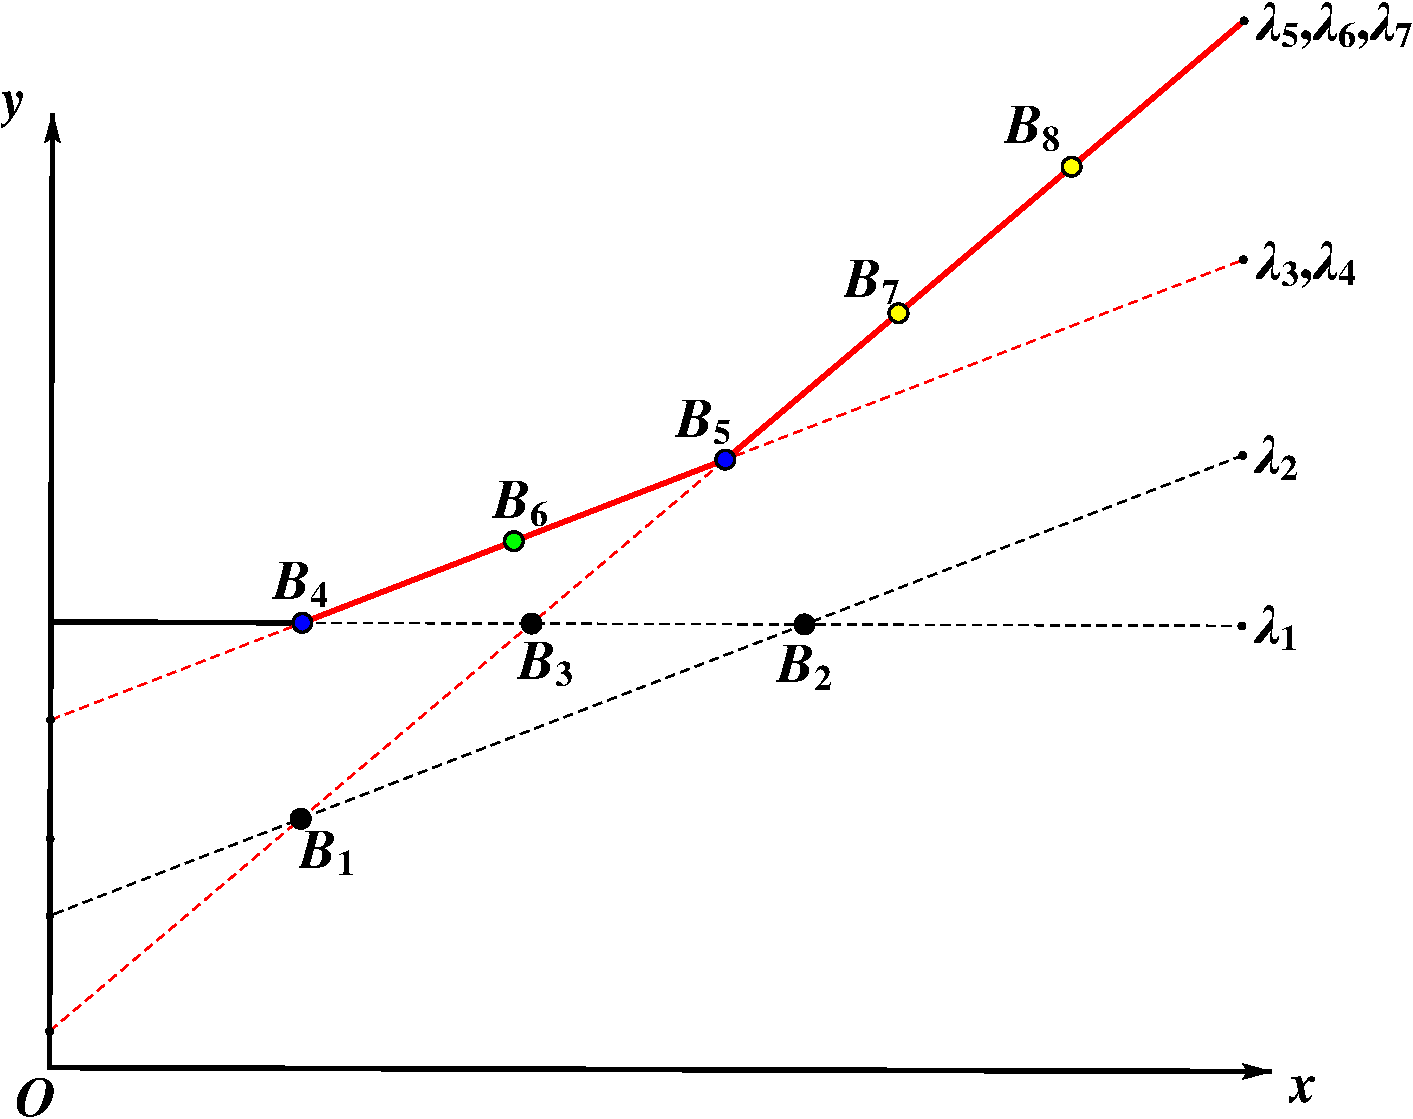
\includegraphics[height=0.9\textheight]{../paper/fig/ps.pdf}
\end{figure}
\end{frame}

\begin{frame}
例1: 只有第一类平衡点
\[
    -x^4f(x+3)+(x+1)f(x)^2+8x^6+27x^5+28x^4+2x^3-x-1=0
\]
\[
    [m+4,2m+1,6]
\]
\[
    m\in \{2,3\} \Rightarrow \overline{m}=3
\]
\end{frame}

\begin{frame}
例2: 第二类平衡点
\[
    x^2f(x)f(x+1)f(x+2)+(1-x^9)f(x)+(x^4-x^9)f(x+1)+2x^9f(x+2)-\sum_{k=0}^{10}{c_k x^k}=0
\]
\[
    [c_0,\cdots,c_{10}]=[1,1,22,57,85,72,35,9,1,10,6]
\]
\[
    [3m+2,m+9,m+9,m+9,10]
\]
\[
    m+9=10 \Rightarrow m=1
\]
\[
    m+9 \ge \max\bbrace{3m+2,10} \Rightarrow m\le 7/2
\]
\[
    \overline{m}=3 \Rightarrow f(x)=x^2=x+1
\]
\end{frame}

\begin{frame}
$n$阶展开方法:
\[
    f(x)=F\sbrace{x,m,u\up n}=\sum_{k=0}^{n-1}{u_k x^{m-k}}+\OO\sbrace{x^{m-n}}
\]
\[
    \OO\sbrace{x^n}=\left\{
    \begin{array}{cl}
    \text{次数不超过}\,n\,\text{的多项式} & n\ge 0, \\
    0                                    & n<0 .
    \end{array}
    \right.
\]
\[
\begin{split}
    0&=\sum_{k=0}^l{\mbrace{a_k(x)\prod_{i=0}^r{f^{\gamma_{ki}}(x+i)}}}\\
    &=F\sbrace{x,\sigma m+\delta,\Omega\up{n}}\\
    &=\Omega_0 x^{\sigma m+\delta}+\cdots+\Omega_{n-1} x^{\sigma m+\delta-n+1} \\
    &+\OO(x^{\sigma m+\delta-n})
\end{split}
\]
\end{frame}



\begin{frame}
例3: 第三类平衡点, 平衡点有解 
\[
    (x+2)f(x)-(x-1)f(x+1)=0
\]
\[
    [m+1,m+1]
\]
\[
    f(x)=u_0 x^m + u_1 x^{m-1} + \OO(x^{m-2})
\]
\[
    (-u_0 m+3u_0)x^m+\OO(x^{m-1})=0
\]
\[
    \overline{m}=3 \Rightarrow f(x)=c(x^3-x)
\]
\end{frame}

\begin{frame}
例4: 第三类平衡点, 平衡点无解
\[
    -2x^5f(x)f(x+2)+x^4f(x)^2+(2x^5-x^4)f(x+1)^2-\sum_{k=0}^{22}{c_k x^k}=0
\]
$[c_0,\cdots,c_{22}]$=[0, 0, 0, 0, 1, 2046, 10140, 22340, 28095, 20730, 7788, 6120, 30600, 84180, 151164, 199504, 199710, 151380, 85560, 35136, 10035, 1830, 170]
\[
    [2m+5,2m+4,2m+5,22]
\]
\[
    \Omega_3 = 2m^2u_0^2-3mu_0^2-2u_0u_1
\]
只有当$2m+5\le 22+3$时, $\Omega_3$对应的项才会和次数为22的项相加, 使得$\Omega_3$的值有可能为零, 从而
\[
    2m+5 \le 22+3 \Rightarrow m\le 10 \Rightarrow f(x)=\pm (x^{10}-1)
\]
\end{frame}

\subsection{$n$阶展开方法在双曲正切方法中的应用}
\begin{frame}{$n$阶展开方法在双曲正切方法中的应用}
例5: 双曲正切方法
\[
    u(u_t+u_{xxx})+pu_x u_{xx}=0
\]
\[
    \mbrace{2m+1,2m+3,2m+3}
\]
\[
    \Omega_0=-{{{a}_{0}}}^{2}\,m\,\left( m\,p+m+2\right) \,\left( m+1\right) \,{k}^{3}
\]
\[
    m=\frac{-2}{p+1}
\]
\[
    u(\xi)=\sum_{k=0}^m{a_k \tanh^k(\xi)}, \xi = kx+ct
\]
$p=-3 \Rightarrow m=1$
\[
    \left\{ c=-4\,{k}^{3},{{a}_{0}}=0\right\}
\]
$p=-5/4\Rightarrow m=8$
\[
\begin{array}{l}
c=16\,{k}^{3},{{a}_{0}}={{a}_{8}},{{a}_{2}}=-4\,{{a}_{8}},{{a}_{4}}=6\,{{a}_{8}},{{a}_{6}}=-4\,{{a}_{8}},\\ 
a_1=a_3=a_5=a_7=0
\end{array}
\]
\end{frame}

\begin{frame}{$n$阶展开方法在\Painleve{}展开法中的应用}
例6: \Painleve{}展开法 
\[
    u(u_t+u_{xxx})-3u_x u_{xx}=0
\]
\[
    \mbrace{2m+1,2m+3,2m+3} 
\]
\[
    \Omega_0=2m(m^2-1)u_0^2f_x^3 \Rightarrow m=1
\]
\[
    u=\frac{F(t)\sqrt{f_x}}{f}
\]
\end{frame}